Afin d'étudier la formation planétaire et les interactions avec le disque de gaz, j'ai utilisé un code de simulation N-corps, qui permet de regarder l'évolution d'un nombre arbitraire de corps orbitant autour d'un astre central \citep{chambers1999hybrid}. 

Ce choix est apparu naturellement. Au début de ma thèse j'ai fait quelques simulations hydrodynamiques avec le code Genesis développé par Arnaud Pierens. J'ai rapidement constaté que ce genre de simulations, bien que modélisant de manière poussée le disque, ne permettait pas d'étudier de manière approfondie la dynamique planétaire. Le temps de calcul nécessaire pour une simulation limite en effet grandement le nombre de corps ainsi que la durée d'intégration. J'ai donc souhaité me tourner vers un code N-corps, afin de privilégier la dynamique planétaire, et de modifier ce programme afin d'y inclure les effets d'un disque de gaz sur la dynamique planétaire. 

J'ai ainsi gagné en temps de calcul, et j'ai ouvert un vaste champ d'investigation sur les paramètres du disques, le nombre de corps en interaction, me permettant de faire des systèmes planétaires très divers, parfois avoir plusieurs centaines d'embryons pour plusieurs millions d'années, chose impossible dans les simulations hydrodynamiques du début de ma thèse où 20 corps pendant quelques dizaines de milliers d'années était un maximum. 

Ce choix a bien entendu introduit son lot d'incertitudes et d'approximations qui sont discutés dans la partie \refsec{sec:discussion}. La présente section a pour but de présenter le code N-corps que j'ai utilisé ainsi que les différents effets du disque que j'ai modélisé. J'ai avant tout souhaité présenter les parties qui ont des conséquences sur la physique du disque, que ce soit en terme de choix d'un modèle particulier, ou de limitations numériques qu'il est bien de garder à l'esprit quand on interprète les résultats.

\section{Présentation de mercury}
Le code N-corps choisi est le code \textbf{mercury} \citep{chambers1999hybrid}. Ce code offre la possibilité de choisir un algorithme parmi 5 différents (BS, BS2, RADAU, MVS et HYBRID), ayant des propriétés diverses. Dans le cadre de ma thèse, je n'ai utilisé que l'algorithme HYBRID, qui utilise l'algorithme MVS la plupart du temps, mais change pour l'algorithme BS2 lors de rencontres proches. Il est possible de déterminer à quel moment on considère qu'une rencontre est "proche" dans le fichier de paramètre de programme, j'ai laissé le paramètre par défaut. 

La raison de ce changement est assez simple. MVS est un algorithme symplectique, c'est à dire à pas de temps constant, dans lequel on défini un hamiltonien que l'on résout pour faire évoluer les orbites. La conservation de l'énergie est moins bonne que pour un algorithme à pas de temps adaptatif, mais le point très important est que cette conservation de l'énergie est bien meilleure au cours du temps. C'est à dire que là où les algorithmes tels que BS, BS2 et RADAU verront leur erreur sur l'énergie augmenter au cours du temps, les algorithmes symplectiques vont eux voir leur erreur rester plus ou moins constante au cours du temps. 

Dans le cadre de mes simulations, j'ai accordé une importance limitée aux variations d'énergie, étant donné que les couples que l'on rajoute pour simuler la présence du disque de gaz font que l'énergie n'est pas conservée pour une planète donnée. Cependant, il est important de bien résoudre les orbites et c'est ce point qui est le plus crucial ici. En effet, quelques tests ont permis de contraindre le pas de temps minimal qu'il est nécessaire d'avoir en fonction de la distance orbitale d'une planète. La contrainte de pas de temps dans mes simulations vient donc d'une distance minimale en dessous de laquelle les orbites ne sont pas correctement calculées. Cette limite, afin d'éviter tout problème, est choisie pour être en dessous du bords interne du disque de gaz que je défini.

\section{Algorithmes d'intégration}
Dans mercury, il y a cinq algorithmes différents à notre disposition :
\begin{itemize}
\item MVS \citep{wisdom1991symplectic} : un code symplectique\footnote{Basiquement, un code symplectique est un code qui conserve parfaitement l'énergie de par sa définition en terme d'hamiltoniens.}, c'est-à-dire qui conserve l'énergie au cours du temps et dont le pas de temps est fixe (c'est le seul à avoir un pas de temps fixe)
\item BS \citep{stoer1980introduction} : un algorithme à pas de temps variable, réputé robuste et plutôt long à tourner.
\item BS2 \citep{press1992numerical} : Basé sur BS, il présente l'inconvénient de ne pas fonctionner pour les systèmes non conservatifs. Il est censé être deux fois plus rapide que BS.
\item RADAU \citep{everhart1985efficient} : Ne fonctionne pas bien pour les rencontres proches et les orbites très excentriques. Est censé être deux à trois fois plus rapide que BS.
\item HYBRID \citep{chambers1999hybrid} : Ce code utilise MVS en temps normal, puis lors d'une rencontre proche, utilise BS2 afin de résoudre correctement les orbites.
\end{itemize}

Il y a donc principalement deux catégories : les intégrateurs symplectiques où le paramètre fixe est le pas de temps ($h=\cte$) et les intégrateurs N-corps où le paramètre est la précision en terme de conservation d'énergie d'un pas de temps à l'autre (le pas de temps n'étant pas fixe). Ici, seuls MVS et HYBRID utilisent une partie symplectique alors que BS, BS2 et RADAU sont purement N-corps.

\bigskip

On défini le Hamiltonien $H$ de notre problème N-corps comme étant la somme des énergies cinétiques et potentielles de chaque corps : 
\begin{align}
H &= \sum_{i=1}^N\frac{{p_i}^2}{2m_i} -G\sum_{i=1}^N\sum_{j=i+1}^N\frac{m_im_j}{r_{ij}}
\end{align}
où $m_i$ est la masse du corps $i$, $p_i$ son impulsion et $r_{ij}$ la séparation entre les corps $i$ et $j$.

Un intégrateur symplectique est un intégrateur qui au lieu d'appliquer directement le hamiltonien $H$ sur le système, va séparer ce dernier en deux (ou plusieurs parties) et appliquer ces sous-hamiltoniens successivement. Un intégrateur symplectique résoud donc le problème de manière approchée en négligeant les termes croisés des sous-hamiltoniens.

Afin de minimiser l'erreur dû à cette approximation, il faut choisir judicieusement la séparation du hamiltonien afin d'avoir une partie dominante par rapport à l'autre.

Par définition, un algorithme symplectique conserve l'énergie au cours du temps, même si l'énergie fluctue au cours du temps autour d'une valeur moyenne. 

Les intégrateurs symplectiques ont deux avantages importants sur les intégrateurs classiques : 
\begin{enumerate}
\item Les fluctuations \og instantanées\fg de l'énergie dues à un algorithme symplectiques sont plus grandes que celles d'un algorithme N-corps, mais à la différence de ces derniers, l'erreur ne croit pas au cours du temps \reffig{fig:energy_error}.
\item Ils sont moins couteux en temps de calcul, en particulier quand la majeure partie de la masse est contenue dans un seul corps (bien adapté pour l'étude d'un système planétaire autour d'une étoile donc).
\end{enumerate}

\begin{figure}[htb]
\centering
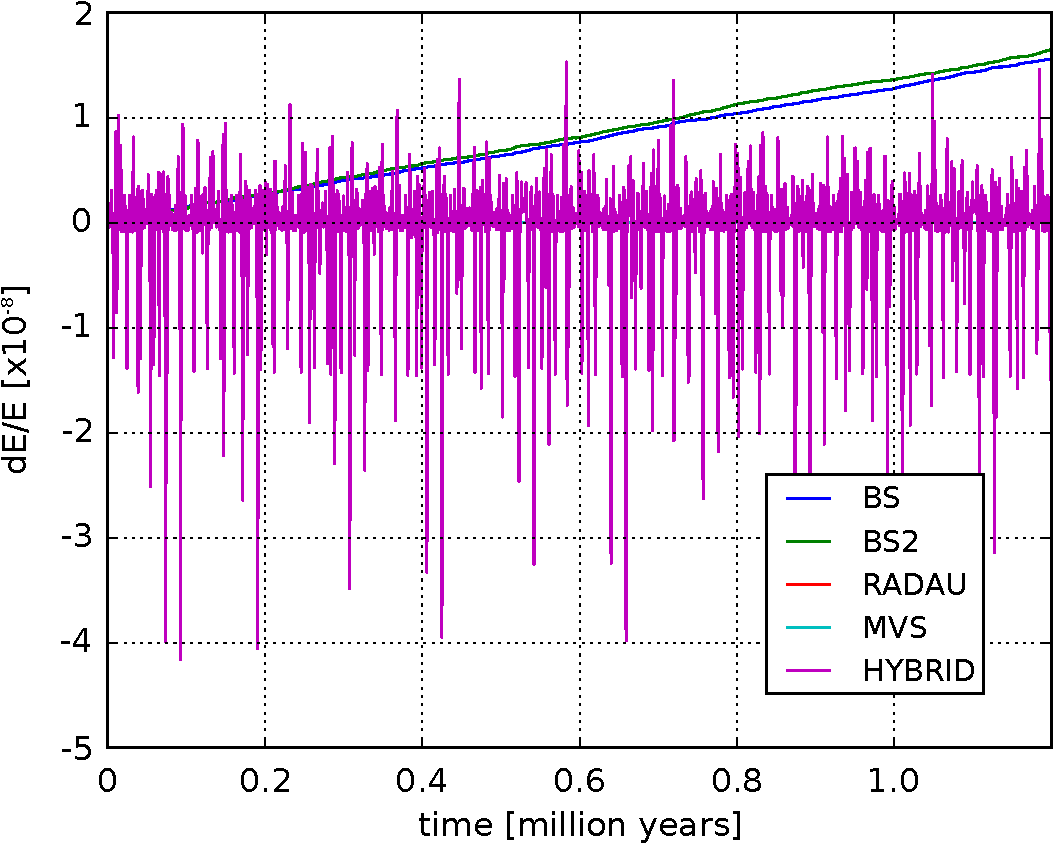
\includegraphics[width=0.65\linewidth]{figure/energy_error.pdf}
\caption{Évolution de l'erreur au cours du temps pour une simulation contenant trois planètes d'une masse terrestre chacune, cette simulation étant lancée successivement avec chacun des algorithmes disponibles dans \textbf{Mercury}.}\label{fig:energy_error}
\end{figure}

Les algorithmes symplectiques ont cependant un inconvénient. Le pas de temps fixe d'un intégrateur symplectique ne permet pas de résoudre correctement les rencontres proches entre les corps du système. Chaque fois que le pas de temps d'un algorithme symplectique est changé, son hamiltonien change aussi, et entraine une variation d'énergie du système (dont l'énergie va osciller autour d'une nouvelle valeur moyenne). 

\bigskip

Nous cherchons maintenant à déterminer l'algorithme le plus approprié pour notre étude. Nous souhaitons faire évoluer un système avec plusieurs dizaines d'embryons planétaire pour plusieurs millions d'années, le système n'étant pas conservatif à cause des divers effets du disque que nous implémentons. 

Nous souhaitons résoudre correctement les orbites, mais avoir un temps de calcul raisonnable. 

La première contrainte est la dissipation. En effet, notre système n'est pas conservatif. Tous les algorithmes N-corps disponibles (BS, BS2 et RADAU) ne fonctionnent donc pas correctement, ces derniers réclament un pas de temps extrêmement faible qui n'est pas représentatif de la précision demandée pour l'intégration N-corps, la variation d'énergie numérique étant masquée par la variation d'énergie induite par les effets du disque. 

Il nous reste les algorithmes MVS et HYBRID. La deuxième contrainte, ce sont les rencontres proches et les collisions. Nous savons qu'un algorithme symplectique ne les traite pas correctement, et si c'est une erreur négligeable dans le cas où il y en a peu, ça ne l'est absolument plus dans notre cas, le nombre de rencontre proche pouvant être très important, notamment dans la phrase d'accrétion en début de simulation. L'algorithme MVS ne parait donc pas adapté contrairement à HYBRID qui a été construit pour être à la fois symplectique et gérer correctement les rencontres proches moyennant une erreur plus importante lors du changement d'algorithme. 

L'algorithme HYBRID est l'algorithme MVS, à pas de temps constant la majorité du temps. Il a donc les avantages d'un algorithme symplectique, à savoir la conservation de l'énergie et la rapidité d'exécution. Lors de rencontres proches (déterminées par une distance minimale d'approche entre deux corps, soit en rayon de Hill, soit en nombre de pas de temps), l'algorithme BS2 est utilisé, le pas de temps devient donc variable afin de résoudre correctement la rencontre et éventuellement la collision. Une fois fini, c'est de nouveau MVS qui prend le relai. 

Dans notre cas, plusieurs approximations sont faites : 
\begin{itemize}
\item L'algorithme BS2 ne fonctionne que pour les systèmes conservatifs. On suppose que la variation d'énergie induite par la migration est totalement négligeable pendant le bref labs de temps de la rencontre proche
\item Le nombre de collisions est suffisamment faible pour que les propriétés symplectiques de l'intégrateur soient conservées. On suppose de plus que les variations d'énergies induites par ce biais sont négligeables devant la dissipation induite par le disque (qui est de l'ordre de l'énergie initiale du système planétaire)
\end{itemize}

Il reste alors une chose à déterminer, c'est le pas de temps fixe que l'on doit choisir afin de résoudre correctement les orbites. Pour cela on se place dans un cas simplifié, sans les effets du disque, et on souhaite savoir la condition sur le pas de temps afin que l'orbite soit correctement calculée. 

On ne s'intéresse qu'aux orbites internes qui sont limitantes au niveau du pas de temps en raison de leur période réduite. Pour une planète à une distance de $0.1\unit{UA}$ du soleil, la période orbitale est de 11 jours environ.

On réalise deux tests. Dans le premier test, on fait évoluer une planète de $1\mearth$ totalement isolée. On fait varier son demi-grand axe et son excentricité et on regarde comment évolue la conservation de l'énergie. Étant donné qu'avec un algorithme symplectique l'énergie oscille au cours du temps, on prend la valeur moyenne de la variation d'énergie, moyenne effectuée sur une centaine de valeurs.

Dans un deuxième test, on procède exactement de la même manière, à ceci près qu'on place une planète de $1\unit{M_\text{jup}}$ à $5\unit{UA}$. 

\reffig{fig:accuracy_maps} montre l'évolution de la conservation de l'énergie dans ces deux tests pour deux pas de temps différents, $h=1\unit{jour}$ et $h=0.4\unit{jour}$. Pour un pas de temps donné, nous ne pouvons pas donner simplement de position en dessous de laquelle l'orbite n'est pas correctement résolue. L'excentricité a une influence. En effet, la distance minimale entre l'étoile et la planète se situe au périhélie, mais suivant l'excentricité, la planète passera plus ou moins de temps au périastre. Ainsi, une très grande excentricité va diminuer drastiquement le temps passé au périastre, pour un périastre donné. 

\begin{figure}[htb]
\centering
\subfloat[$h=1\unit{jour}$ sans Jupiter]{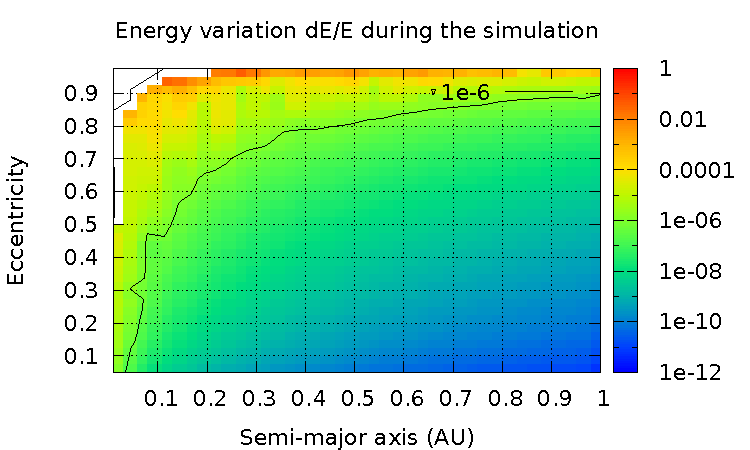
\includegraphics[width=0.49\textwidth]{figure/accuracy_10_one.pdf}}\hfill
\subfloat[$h=1\unit{jour}$ avec Jupiter]{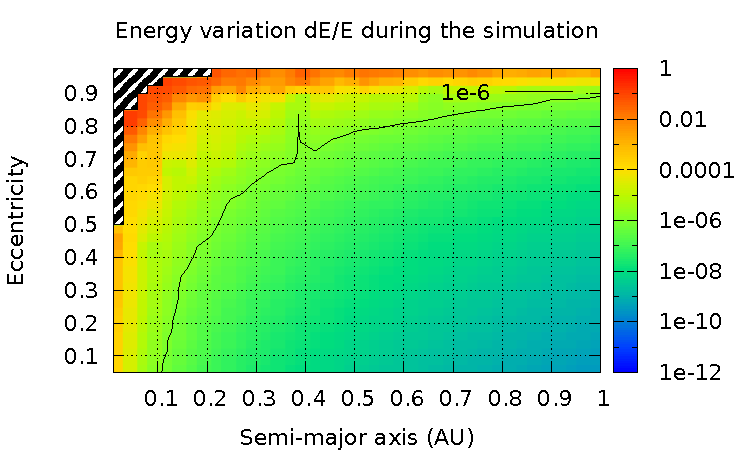
\includegraphics[width=0.49\textwidth]{%
figure/accuracy_10_jup.pdf}}

\subfloat[$h=0.4\unit{jour}$ sans Jupiter]{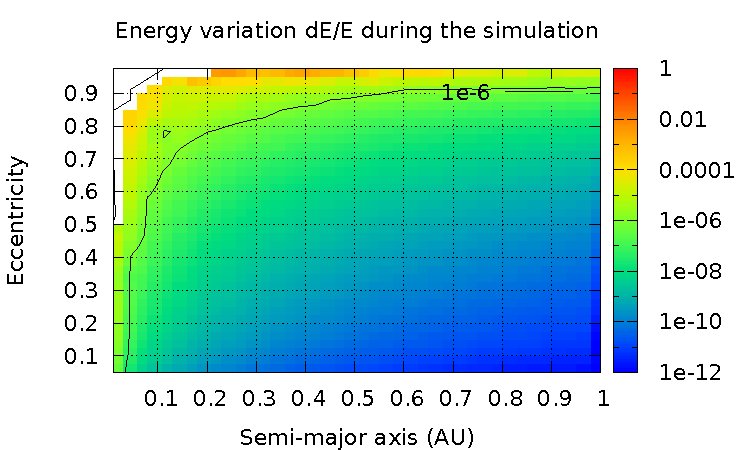
\includegraphics[width=0.49\textwidth]{figure/accuracy_04_one.pdf}}\hfill
\subfloat[$h=0.4\unit{jour}$ avec Jupiter]{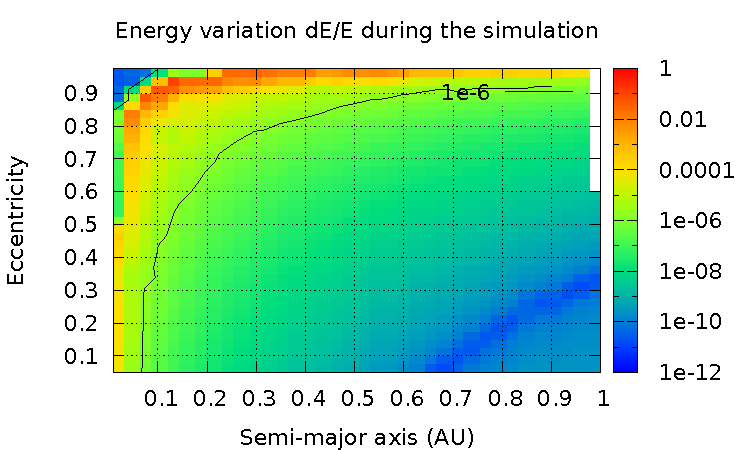
\includegraphics[width=0.49\textwidth]{%
figure/accuracy_04_jup.pdf}}


\caption{Tests pour $h=1\unit{jour}$ et $h=0.4\unit{jour}$ de la conservation de l'énergie pour une planète de $1\mearth$ isolée ou avec un compagnon de la taille de Jupiter. Les cartes montrent la conservation de l'énergie pour différentes valeurs du demi-grand axe $a$ et de l'excentricité $e$. La ligne noire correspond à un $\dif E/E=10^{-6}$, valeur en dessous de laquelle on considère que la précision sur l'orbite est suffisante. La partie hachurée correspond à la collision de la planète interne avec l'étoile centrale donc le rayon est $R_\star=0.005\unit{UA}$.}\label{fig:accuracy_maps}
\end{figure}

Si un pas de temps plus grand ($h=1\unit{jour}$) semble convenir pour une planète isolée, la conservation de l'énergie est différente dans le cas avec des perturbations gravitationnelles (cas avec Jupiter). À $0.1\unit{UA}$, qui correspond au bord interne, zone particulièrement importante pour notre étude, ce pas de temps ne convient plus. Dès que l'excentricité augmente un peu, la précision sur l'orbite diminue, et les orbites les plus internes,  ne sont pas correctement résolue.

Même si le disque amortie les excentricités, nous souhaitons résoudre correctement les orbites légèrement excentriques, même au bord interne à $0.1\unit{UA}$. Le pas de temps qui nous semble convenir le mieux à notre problème est $h=0.4\unit{jour}$. C'est donc celui que nous utiliserons par défaut.

Un moyen mnémotechnique pour calculer le pas de temps minimal pour une simulation est de considérer qu'il faut résoudre l'orbite la plus proche avec un minimum de $10$ pas de temps. Ceci n'est valable que dans l'approximation où l'excentricité n'est pas trop élevée ($e<0.4$). Si nous faisons ce calcul ici, nous obtenons qu'avec un demi-grand axe minimal de $a=0.1\unit{UA}$ et une excentricité maximale de $e=0.4$, la distance minimal d'approche est $q=0.06$. La période d'une orbite $a=0.06$ est de $5\unit{jours}$ environ, ce qui donne un pas de temps maximal de $h=0.5\unit{jour}$. 


\section{Mode d'emploi du code N-corps modifié}
À part la première section qui donne quelques détails techniques, le but de cette partie est de présenter les différentes options du code modifié. Ces options sont lues à partir d'un fichier commun \textbf{disk.in}. Si une option n'est pas présente, la valeur par défaut sera lue à partir du code. Le fichier \textbf{disk.out} récapitule toutes les valeurs de toutes les options et paramètres importants du code. 

\begin{remarque}
Il est possible de mettre des commentaires dans le fichier \textbf{disk.in}, que ce soit pour commenter une ligne entière, ou pour mettre en fin de ligne après un paramètre, à l'aide du caractère \og !\fg exactement comme en Fortran90.
\end{remarque}

\subsection{Note technique}
Le code est en grande partie le code mercury \cite{chambers1999hybrid}. Les effets du disque ont été inclus dans la partie \textbf{mfo\_user} prévue pour inclure des effets propre à chaque utilisateur. 

Pour autant, le code a été conçu de manière modulaire en portant une attention particulière au temps d'exécution et à la souplesse d'utilisation. La plupart des effets sont désactivables par une simple option dans un fichier de paramètre spécifique au effets du disque \textbf{disk.in}. 

Prenons un exemple. Le couple exercé par le disque sur la planète peut être issus des formules de \cite{paardekooper2011torque}, ou bien suivre plusieurs lois artificielles permettant de tester certains effets dans des cas simplifiés. Pour autant, cette souplesse d'utilisation ne se fait pas au détriment de la célérité du code car au lancement du code, les options sont lues et des pointeurs de fonctions permettent au code d'exécuter directement la bonne fonction lors de l'intégration, sans avoir à tester à chaque pas de temps quelle fonction doit être lancée. 

\bigskip

Un programme externe, nommé \textbf{test\_disk} permet d'effectuer des tests unitaires sur différentes fonctions, afin de vérifier quand bon nous semble que chaque fonction n'est pas perturbée par les autres et donne des résultats corrects à la fois physiquement et numériquement.

\subsection{Paramètres divers}
Ici je regroupe des paramètres du disque qui nécessitent simplement une valeur : 
\begin{verbatim}
b/h = 0.6
adiabatic_index = 1.4
mean_molecular_weight = 2.35
disk_edges = 0.1 100.
sample = 800
\end{verbatim}

\textbf{b/h} est la longueur de lissage du potentiel gravitationnel d'une planète (qui diverge dans les simulations hydrodynamiques et qui est un paramètre des formules de \cite{paardekooper2011torque}.

\textbf{adiabatic\_index} est l'indice adiabatique $\gamma$ comme son nom l'indique. De même, \textbf{mean\_molecular\_weight} est la masse moléculaire moyenne $\mu$.

\textbf{disk\_edges} défini les deux extrémités du disque, les bords internes et externes.

\textbf{sample} défini le nombre de points qu'auront les profils radiaux des différents paramètres du disque. Ces points ne sont pas répartis uniforméments, il y a plus de points au bord interne qu'au bord externe, afin d'avoir une évolution plus fine des paramètres en fonction du rayon.

\subsection{Densité de surface}
\textbf{surface\_density} permet de définir le profil en loi de puissance pour la densité de surface : 
\begin{verbatim}
surface_density = 500 0.5
\end{verbatim}
Ici, on a défini le profil suivant : 
\begin{align*}
\Sigma(R) &= 500. \cdot R^{-0.5} \unit{g/cm^2}
\end{align*}

Mais il est aussi possible de donner un profil tabulé de densité de surface en fonction du rayon en paramètre d'entrée, en spécifiant le paramètre suivant : 
\begin{verbatim}
surface_density = manual
\end{verbatim}
Ainsi, le profil de densité de surface sera lu à partir du fichier \textbf{surface\_density\_profile.dat} qui doit être constitué de deux colonnes, la première étant la valeur du rayon en AU, et la deuxième la densité de surface en \unit{g/cm^2}. Les lignes doivent être classées par ordre croissant de distance orbitale. (les premières lignes étant les points les plus proches de l'étoile, et les dernières les points les plus lointains. 

\begin{remarque}
Une interpolation sera réalisée si la discrétisation du fichier d'entrée est différente de celle du code.
\end{remarque}

\bigskip

À ceci s'ajoute un paramètre supplémentaire : 
\begin{verbatim}
inner_smoothing_width = 0.05
\end{verbatim}

Ce paramètre représente la longueur d'amortissement de la densité de surface au bord interne du disque, afin que la densité de surface au bord interne soit très faible. Cette longueur est exprimée en pourcentage de distance orbitale du bord interne ; c'est à dire que si le bord interne est à 0.1 AU, alors dans le cas présent, le lissage sera effectué sur une longueur de 0.005AU

\subsection{Irradiation de l'étoile centrale}
\textbf{is\_irradiation} permet de définir si on veut inclure ou non l'irradiation dans le calcul de l'équilibre énergétique du disque. 

\begin{verbatim}
is_irradiation = 1
disk_albedo = 0.5
r_star = 4.65e-3 ! AU
t_star = 5700 ! K
\end{verbatim}

Les paramètres sont relativement explicite mais pour détailler, \textbf{disk\_albedo} est l'albedo moyen du disque protoplanétaire, il représente le fait qu'une partie de la lumière incidente de l'étoile est directement réfléchie vers l'espace.

\textbf{r\_star} et \textbf{t\_star} sont respectivement le rayon de l'étoile en AU et sa température en Kelvin.

La manière dont est modélisée l'irradiation de l'étoile centrale est détaillée dans \refsec{sec:irradiation}.

\subsection{Viscosité}
Il est possible de définir plusieurs types de viscosité via l'option \textbf{viscosity\_type} : \textbf{constant}, \textbf{alpha} et \textbf{alpha\_dz}.

\subsubsection{constant}
Ce paramètre permet de définir une viscosité $\nu$ constante dans tout le disque. La valeur de la viscosité associée est définie dans le paramètre \textbf{viscosity} en \unit{cm^2/s}.

\begin{verbatim}
viscosity_type = constant
viscosity = 1e15 ! cm^2/s
\end{verbatim}

\subsubsection{alpha}
Ce paramètre permet de définir une viscosité via la prescription alpha de \cite{shakura1973black}. La valeur du paramètre alpha sera lue dans le paramètre \textbf{alpha}. 

\begin{verbatim}
viscosity_type = alpha
alpha = 5e-3
\end{verbatim}

\subsubsection{alpha\_dz}\label{sec:dead_zone}
Ce paramètre permet de définir une viscosité alpha par morceau, permettant de modéliser une dead zone. On aura donc 3 zones avec 3 alpha différents. Pour définir ces zones là, il faut donner dans le paramètre \textbf{alpha\_dz} trois valeurs de $\alpha$ et dans \textbf{radius\_dz} deux valeurs de distance orbitales (en AU) pour définir les bornes de la dead zone.
\begin{verbatim}
viscosity_type = alpha_dz
alpha_dz = 0.005 0.0001 0.005
radius_dz = 1.0 10.0 ! in AU
\end{verbatim}

Quand cette option est activée, une modification au profil de densité est appliquée, afin de modéliser une sous-densité, puis une sur-densité avant et après le bord interne de la zone morte. L'écart maximum de ces \og bumps\fg est de 15\% de la valeur de la densité au bord interne de la zone morte. 

À ceci s'ajoute un lissage des valeurs de $\alpha$ entre la valeur à gauche et la valeur à droite de la transition selon une tangente hyperbolique. La transition s'effectue typiquement sur une longueur égale à 10\% de la position de la transition dans le disque (si la transition est à 1AU, alors la transition a lieu sur 0.1 AU autour de la transition).

\subsection{Opacité}
Afin de pouvoir les comparer, j'ai ajouté au code la possibilité de tourner avec différents modèles pour l'opacité. 

Les différents modèles sont \citep{bell1994FU, zhu2009nonsteady, chambers2009analytic, hure2000transition}

\subsubsection{bell}
\begin{verbatim}
opacity_type = bell
\end{verbatim}

L'opacité est alors calculée en utilisant le modèle fourni par \cite{bell1994FU}. 

\subsubsection{zhu}
\begin{verbatim}
opacity_type = zhu
\end{verbatim}

L'opacité est alors calculée en utilisant le modèle fourni par \cite{zhu2009nonsteady}. 

\subsubsection{chambers}
\begin{verbatim}
opacity_type = chambers
\end{verbatim}

L'opacité est alors calculée en utilisant le modèle fourni par \cite{chambers2009analytic}. Ce modèle est très simplifié et utilisé une opacité constante sur un grand régime de température, pour ensuite faire une transition vers une loi de puissance à très haute température.

\subsubsection{hure}
\begin{verbatim}
opacity_type = hure
\end{verbatim}

L'opacité est alors calculée en utilisant le modèle fourni par \cite{hure2000transition}. 

À la différence de tous les autres modèles que j'ai implémenté, celui de \cite{hure2000transition} est directement une table d'opacité, sans faire intervenir de loi de puissance pour différents régimes. Il n'introduit donc pas d'incertitudes supplémentaire via les loi de puissance qu'il défini. Cette table
d'opacité de Rosseland correspond à la composition suivante $X=0.70$, $Y=0.28$ et $Z=0.02$ et est basée sur
\cite{seaton1994opacities, alexander1994low, henning1996dust}.

En effet, dans le cas qui nous intéresse, c'est à dire la migration planétaire via la formule de \citep{paardekooper2011torque}, l'indice des loi de puissance pour la densité de surface et la température a une très grande influence sur la couple effectif du disque. Et les transitions d'opacités, très marquées lors de la transition des lois de puissance, fait apparaître des zones particulières dans le disque qui n'ont parfois aucune réalité physique mais ont de grandes conséquences sur le résultat des simulations. De même, le lissage qu'elles introduisent masquent certaines zones d'intérêt qui ne sont mises en évidence qu'avec une table d'opacité où tous les effets fins ont été préservés.

\subsection{Turbulence}
Pour activer la turbulence dans le disque, c'est à dire l'effet que la turbulence peut induire sur la migration planétaire, il suffit d'utiliser le paramètre suivant : 
\begin{verbatim}
is_turbulence = 1
\end{verbatim}

La turbulence n'est ici qu'une migration stochastique de moyenne nulle qui perturbe les planètes et leur migration. 

Le modèle utilisé est le même que celui détaillé dans \cite{ogihara2007accretion}. Le principe est de définir un potentiel turbulent dans le disque, fait de la superposition de perturbation individuelle qui ont des modes $m$, temps de vie $t_m$ et position dans le disques différents. 

Dans le cas typique, il y a 100 modes différents dans le disque : 
\begin{align}
\Phi_\text{turb}(R,\phi,t) &= \gamma R^2 \Omega^2 \sum_{k=1}^{100} \Lambda_k(R,\phi,t)
\end{align}
avec 
\begin{align}
\Lambda_k &= \xi_k e^{-\frac{(R-R_k)^2}{{\sigma_k}^2}} \cos\left(m_k \phi -\phi_k - \Omega_k\tilde{t}_k\right) \sin\left(\pi \tilde{t}_k/\Delta t_k\right)
\end{align}

$\xi_k$ est une constante adimensionnée déterminée aléatoirement en suivant une distribution gaussienne.

$R_k$ et $\phi_k$ sont respectivement les coordonnées radiales et azimutales du mode $k$ choisies aléatoirement et de manière uniforme pour l'un entre les bornes du disque, pour l'autre entre $0$ et $2\pi$. 

Chaque mode $k$ possède un nombre de mode $m_k$ déterminée selon une distribution logarithmique entre $m=1$ et $m=150$, le nombre de mode déterminant l'extension radiale et la durée du vie du mode $k$.

$\sigma_k = \pi R_k / 4m_k$ est l'extension radiale de ce mode tandis que $\Omega_k$ représente la vitesse angulaire képlerienne à la position $R=R_k$.

$\Delta t_k=0.2\pi R_k / m_k c_s$ est la durée de vie du mode $k$. 

\bigskip

Les modes apparaissent et disparaissent en fonction de leur temps de vie et sont remplacés afin qu'il y ait toujours 100 modes différents dans le disque à un instant $t$. Chaque mode $k$ est créé à un instant $t_{0,k}$ et se termine quand $\tilde{t}_k = t-t_{0,k} > \Delta t_k$.

\subsection{Migration}
\subsubsection{real}
C'est le cas le plus classique. Il n'y a pas besoin de définir d'autres paramètres, la migration induite par le disque de gaz sera simplement calculée à partir du modèle de \cite{paardekooper2011torque}.

\begin{verbatim}
torque_type = real
\end{verbatim}

\subsubsection{mass\_dependant}\label{sec:mass_dependant}
\begin{figure}[htb]
\centering
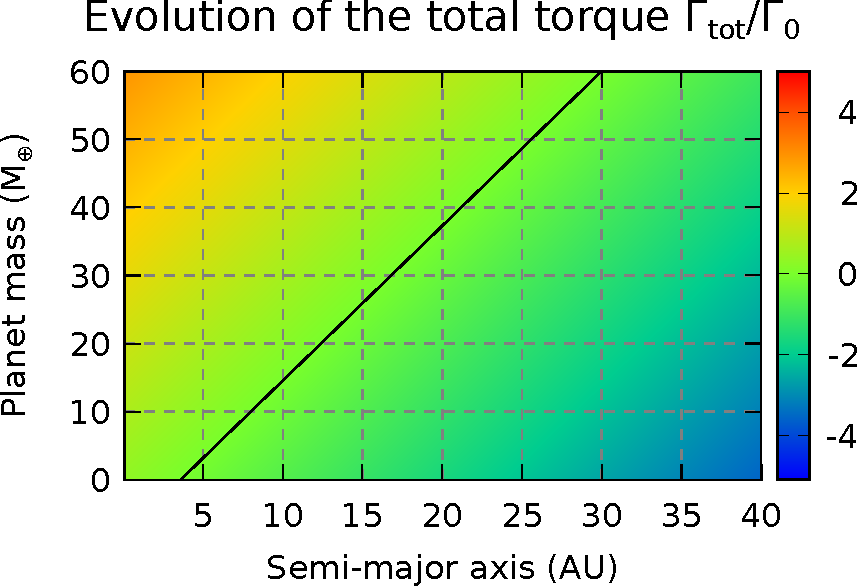
\includegraphics[width=0.65\linewidth]{figure/migration_map/mass_dependant.pdf}
\caption{Cette carte représente l'effet du disque dans le cas de l'option \textbf{mass\_dependant} pour une planète en fonction de sa position en abscisse et de sa masse en ordonnée. La ligne noire représente la zone de couple nul, c'est à dire une zone où la migration de la planète s'arrête.}
\end{figure}

On définit une zone de convergence artificielle qui va dépendre de la masse des planètes. On va donc devoir définir deux bornes en masses et deux bornes en distance orbitale qui vont déterminer cette ligne de couple nul. À l'intérieur (resp. extérieur) de cette séparation virtuelle, la migration sera vers l'extérieur (resp. intérieur).

Ensuite, on défini une pente linéaire plus ou moins importante pour voir à quelle vitesse on va tendre vers la valeur de saturation à mesure qu'on s'éloigne de la zone de convergence. Une pente de $1$ signifie que le couple $\Gamma/\Gamma_0$ augmente de 1 tous les 10 AU.

En résumé, on a ces paramètres suivants à définir : 
\begin{verbatim}
torque_type = mass_dependant

mass_dep_cz_m_max = 30 ! AU
mass_dep_m_max = 60 ! m_earth

mass_dep_cz_m_min = 4 ! AU
mass_dep_m_min = 1 ! m_earth

torque_profile_steepness = 1.0
\end{verbatim}

\subsubsection{linear\_indep}\label{sec:linear_indep}
Même chose que précédemment, on peut définir un couple artificiel qui défini une zone de convergence indépendante de la masse, c'est à dire qu'on ne spécifie que la position de la zone de convergence dans le disque. On a donc : 
\begin{verbatim}
torque_type = linear_indep
indep_cz = 3.0 ! AU
torque_profile_steepness = 1.0
\end{verbatim}

Une pente de $1$ signifie que le couple $\Gamma/\Gamma_0$ augmente de 1 tous les 10 AU.

\begin{figure}[htb]
\centering
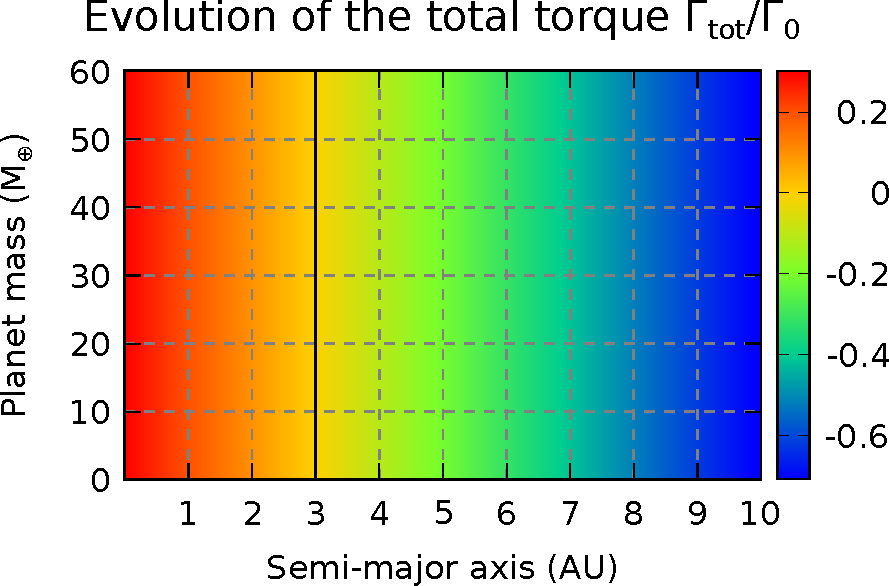
\includegraphics[width=0.65\linewidth]{figure/migration_map/linear_indep.pdf}
\caption{Cette carte représente l'effet du disque dans le cas de l'option \textbf{linear\_indep} pour une planète en fonction de sa position en abscisse et de sa masse en ordonnée. La ligne noire représente la zone de couple nul, c'est à dire une zone où la migration de la planète s'arrête.}
\end{figure}

\subsubsection{tanh\_indep}\label{sec:tanh_indep}
Ici, on défini aussi une zone de convergence indépendante de la masse, mais au lieu d'avoir une évolution linéaire du couple à mesure qu'on s'éloigne de la zone de convergence, on a une tangente hyperbolique qui sature à une valeur que l'on peut donner en paramètre. 

La valeur du couple de saturation défini la valeur absolue du couple vers laquelle on va tendre quand on est très loin de la zone de convergence. Si on est à l'extérieur, ce sera cette valeur de saturation prise négativement, tandis que c'est la valeur positive qui est utilisée à l'intérieur.

On a donc les paramètres suivants à définir : 
\begin{verbatim}
torque_type = tanh_indep
indep_cz = 3.0 ! AU
saturation_torque = 1.0 ! in Gamma_0
\end{verbatim}

\begin{figure}[htb]
\centering
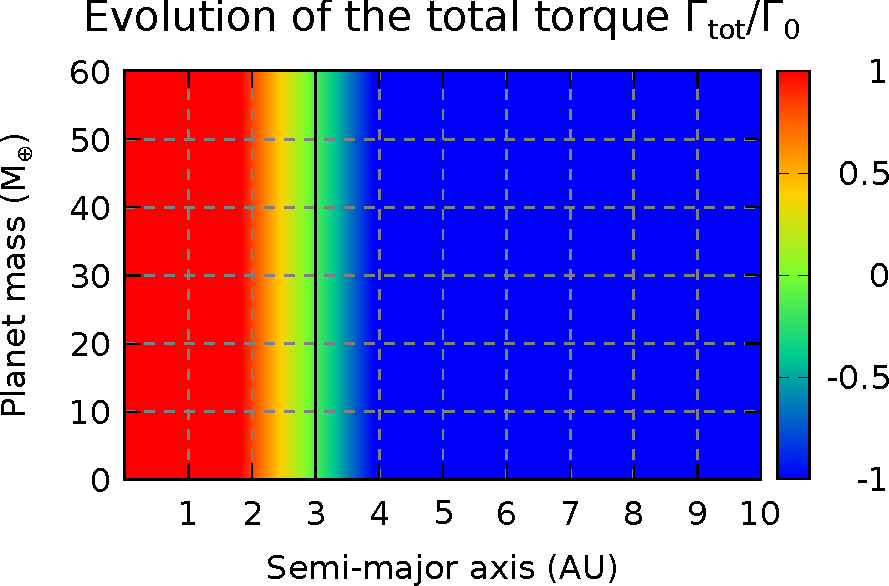
\includegraphics[width=0.65\linewidth]{figure/migration_map/tanh_indep.pdf}
\caption{Cette carte représente l'effet du disque dans le cas de l'option \textbf{tanh\_indep} pour une planète en fonction de sa position en abscisse et de sa masse en ordonnée. La ligne noire représente la zone de couple nul, c'est à dire une zone où la migration de la planète s'arrête.}
\end{figure}

\subsubsection{manual}
Il est aussi possible de rentrer manuellement un couple total en fonction de la position de la planète dans le disque. 

Les valeurs seront alors lues à partir du fichier \textbf{torque\_profile.dat}. La première colonne sera les positions dans le disque en AU tandis que la deuxième colonne sera le couple exercé par le disque en unité de $\Gamma_0$ (c'est à dire que l'effet de la masse de la planète sur la vitesse de migration sera toujours pris en compte dans le code au travers de la dépendance de $\Gamma_0$ en fonction de la masse de la planète et de la masse du disque.

\section{Disque (1+1)D}
Afin de calculer les effets d'un disque de gaz, une modélisation de ce dernier est nécessaire. Le but étant d'avoir une grande souplesse, le disque implémenté est bien entendu très simplifié. Toutes les quantités sont intégrées et invariantes selon la hauteur z et la position azimutale $\theta$ dans le disque, résultant en un modèle radial 1D de toutes les quantités. 

Dans la mesure du possible, les quantités du disque ont été calculées de manière consistante. Je vais présenter dans la suite de manière chronologique comment sont calculées les grandeurs physiques du disque.

\subsection{Profil de densité de surface}
Le profil de densité de surface est défini au début de la simulation comme une loi de puissance de la forme :
\begin{align}
\Sigma(R) &= \Sigma_0 \times R^{-d}
\end{align}
où $\Sigma_0$ est la densité de surface à $1\unit{AU}$ et $d$ l'indice de la loi de puissance. 

Ce profil de densité de surface est défini pour une certaine étendue radiale. On défini donc un bord interne $R_\text{in}$ et un bord externe $R_\text{out}$. Le bord interne est généralement à $0.1\unit{AU}$ et le bord externe à $100\unit{AU}$. 

Afin de calculer les valeurs suivantes, ce disque est échantillonné et toutes les valeurs nécessaires sont ensuite calculées à chacun de ces points. 

\bigskip

Le profil de densité de surface est le paramètre d'entrée le plus important. Il est celui à partir duquel on calcule toutes les autres quantités du disque, température, échelle de hauteur, etc\dots

Le profil étant une loi de puissance, un amortissement est effectué au bord interne du disque afin que la valeur de la densité au bord interne soit proche de zéro. 

Le profil de densité de notre disque de référence (dont nous parlerons plus en détail \refsec{sec:migrations-maps}) est représenté \reffig{fig:fiducial_density}

\begin{figure}[htb]
\centering
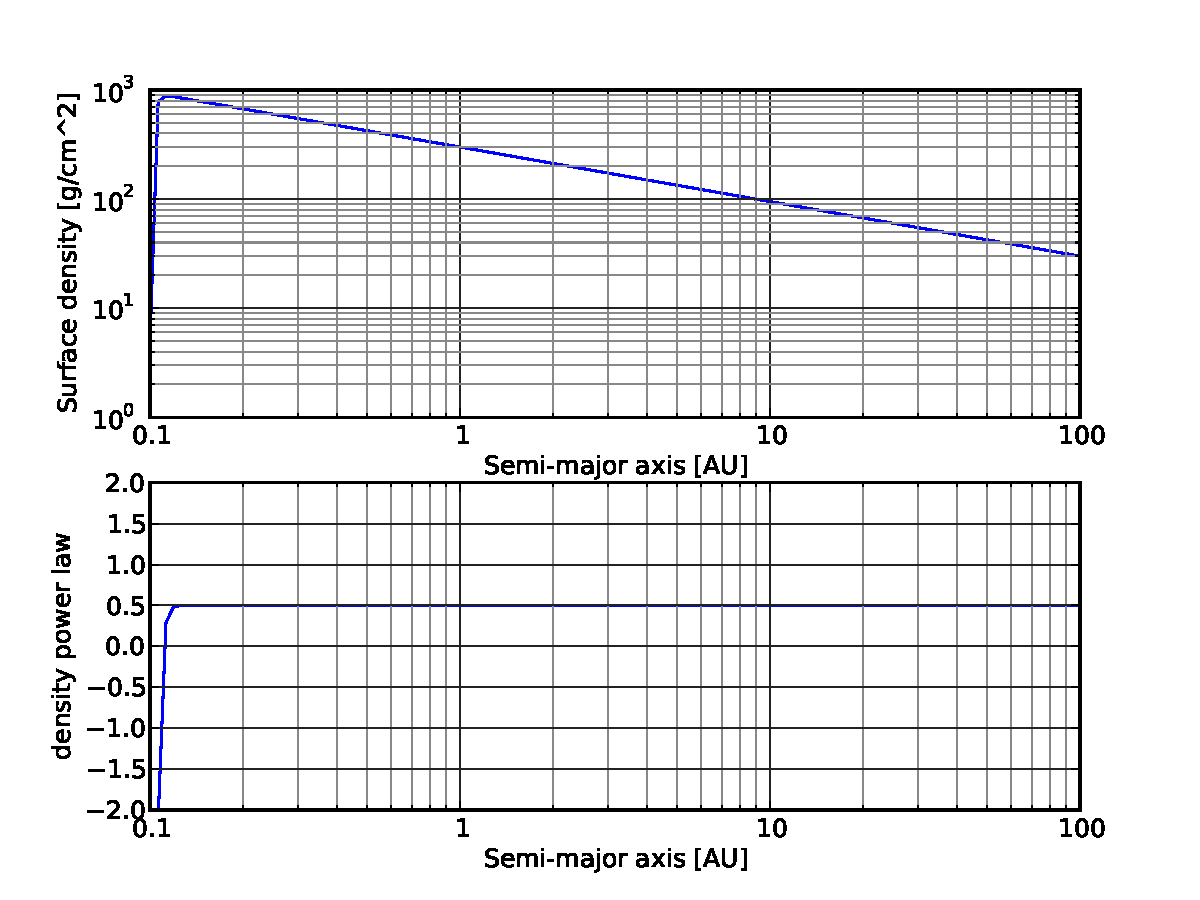
\includegraphics[width=0.75\linewidth]{figure/fiducial_density_profile.pdf}
\caption{Profil de densité de surface pour notre disque de référence \protect\reftab{tab:fiducial_parameters}.}\label{fig:fiducial_density}
\end{figure}

\subsection{Table d'opacité}
Afin de pouvoir calculer le profil de température, on a besoin de choisir un modèle pour l'opacité. Je ne détaillerai pas ici les différents modèles car une étude complète sur le sujet a été effectuée, afin de comprendre l'influence du choix du modèle sur les résultats des simulations. 

Par contre, quel que soit le modèle, on a généralement une dépendance en fonction de la densité et de la température. L'opacité est donc un paramètre de la résolution de l'équation qui nous permet d'avoir la température. L'opacité n'est pas, dans notre modèle, une quantité qu'on fixe \textit{a priori}, mais plutôt un des paramètres de sortie de la résolution de l'équation de l'énergie dans le disque.

%TODO 
\subsection{Profil de température}
Afin de construire le profil de température point par point, on résout, pour chaque position dans le disque définie dans le profile, l'équation de l'énergie \refeq{eq:equation_energie}. 

De manière consistante, cette équation a pour paramètre d'entrée la position, et on cherche à trouver les valeurs de la température $T$, échelle de hauteur $H$, profondeur optique $\tau$, diffusivité thermique $\chi$. Toutes ces valeurs sont fixées une fois qu'un ensemble cohérent de valeurs satisfont l'équation.

Afin de résoudre cette équation du type $f(x)=0$, j'ai utilisé une version modifiée de la méthode \textbf{zbrent} de \textbf{Numerical Recipes} \citep{press1992numerical}

Le profil de température que nous obtenons dans notre disque de référence (dont nous parlerons plus en détail \refsec{sec:migrations-maps}) est représenté \reffig{fig:fiducial_temperature}

\begin{figure}[htb]
\centering
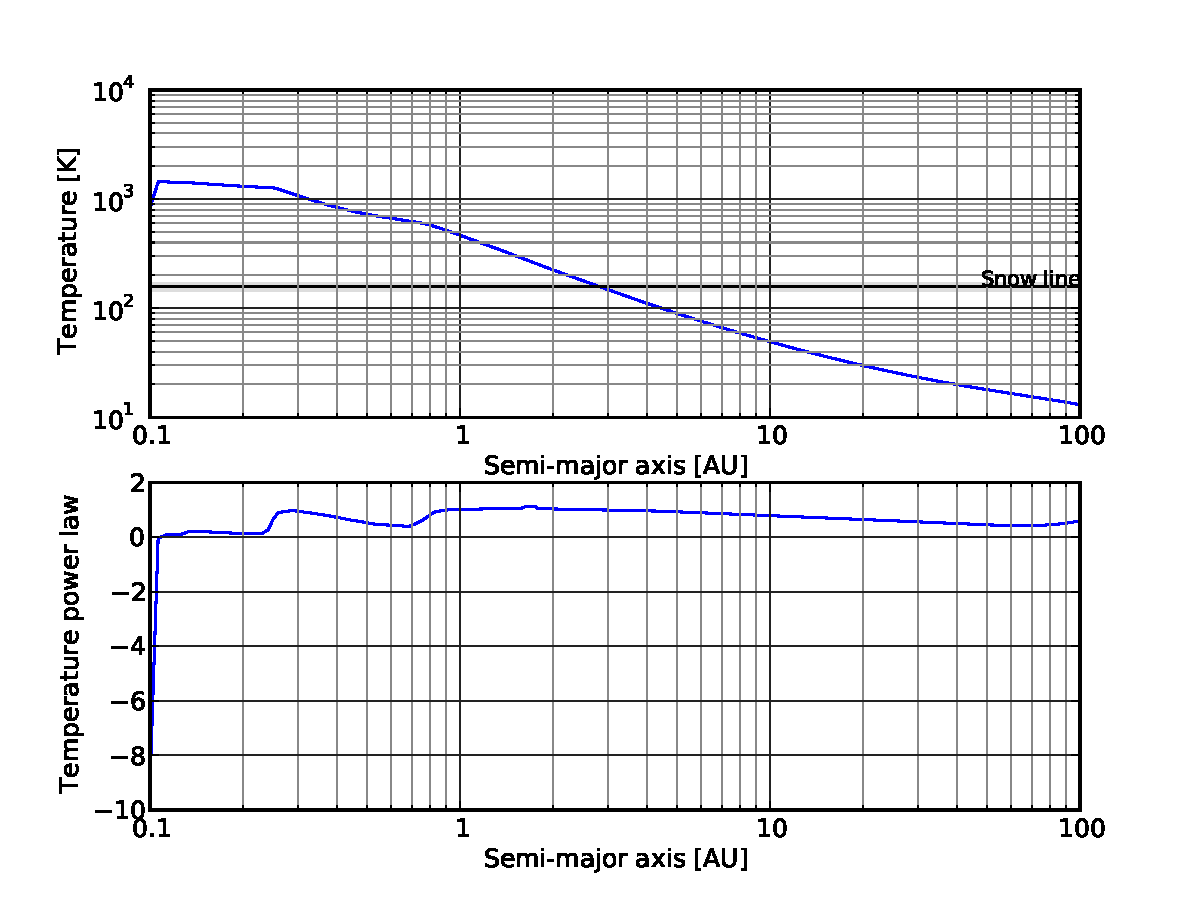
\includegraphics[width=0.75\linewidth]{figure/fiducial_temperature_profile.pdf}
\caption{Profil de température pour notre disque de référence \protect\reftab{tab:fiducial_parameters}.}\label{fig:fiducial_temperature}
\end{figure}

%TODO 
\section{Migration type I}
La migration de type I est implémentée dans le code en utilisant le modèle 1D de disque, qui définit pour toute position du disque, une température, une densité de surface, et tous les autres paramètres nécessaires comme l'échelle de hauteur. En utilisant ces paramètres, on obtient ainsi le couple qu'exerce le disque sur la planète en fonction de sa masse et de sa position via la formule semi-analytique de \cite{paardekooper2011torque}. 

Les deux différences principales entre le cadre du modèle de \cite{paardekooper2011torque} et le disque que j'ai modélisé, c'est que dans mon cas je n'ai pas un profil de température en loi de puissance (avec une seule loi de puissance), mais j'ai une loi de puissance définie point par point. C'est à dire que pour chaque zone du disque, la température est calculée de manière cohérente avec les autres paramètres du disques, et que l'indice de la loi de puissance correspondante est calculée en fonction des températures autour.

La deuxième différence est que j'ai un profil pour l'échelle de hauteur $H$ et le rapport d'aspect $h=H/R$ du disque au lieu d'avoir un rapport d'aspect constant pour tout le disque.

\bigskip

De plus, certaines erreurs se sont glissées dans ce papier. \cite[appendice A]{bitsch2011range} fait remarquer en particulier qu'il manque un facteur 4 dans l'équation (33). Ainsi, la formule que j'ai utilisé pour calculer la conductivité thermique $\chi$ est :
\begin{align}
\chi &= \frac{16\gamma (\gamma-1) \sigma T^4}{3\kappa \rho^2 H^2\Omega^2}
\end{align}

Il y a aussi une erreur dans l'équation (35) car le disque se refroidit par la surface supérieur et la surface inférieure. Mais comme j'utilise dans mon code une équation de l'énergie \refeq{eq:equation_energie} un peu plus complexe où j'ai tenu compte de ce fait là, cette erreur n'a pas d'incidence sur le calcul du couple.

Les formules nous donnent alors un couple exercé par le disque sur la planète. 

À partir de ce couple, on définit un temps de migration $t_\text{mig}$ comme : 
\begin{align}
t_\text{mig} &= \frac{J}{2\Gamma}
\end{align}
où $J$ est le moment angulaire total de la planète et $\Gamma=\dot{J}$ est le couple total exercé par le disque sur la planète.

L'accélération due à la migration $\vect{a_\text{mig}}$ est alors donnée par :
\begin{align}
\vect{a_\text{mig}} &= \frac{\vect{v}}{t_\text{mig}}
\end{align}
où $\vect{v}$ est la vitesse instantanée de la planète.

\section{Amortissement de e et I}
L'amortissement de l'eccentricité $e$ et de l'inclinaison $I$ d'une planète plongée dans un disque protoplanétaire est modélisée dans le code via les formules de \cite[eq. (9), (11) et (12)]{cresswell2008three} : 
\begin{subequations}
\begin{align}
t_\text{wave} &= \frac{M_\star}{m_p}\frac{M_\star}{\Sigma_p {a_p}^2}\left(\frac{H}{r}\right)^4{\Omega_p}^{-1}\\
t_e &= \frac{t_\text{wave}}{0.780}\left[1-0.14\left(\frac{e}{H/r}\right)^2 + 0.06 \left(\frac{e}{H/r}\right)^3 + 0.18\left(\frac{e}{H/r}\right)\left(\frac{i}{H/r}\right)^2\right]\\
t_i &= \frac{t_\text{wave}}{0.544}\left[1-0.30\left(\frac{i}{H/r}\right)^2 + 0.24 \left(\frac{i}{H/r}\right)^3 + 0.14\left(\frac{e}{H/r}\right)^2\left(\frac{i}{H/r}\right)\right]
\end{align}
\end{subequations}

L'amortissement de $I$ est arrêté quand l'inclinaison descend en dessous de $I<5\cdot 10^{-4}\unit{rad}$ afin d'empêcher les planètes d'être parfaitement dans le plan $(x,y)$, essentiellement pour empêcher des problèmes numériques.

%TODO 
\section{Effet de l'excentricité sur le couple de corotation}
Afin de tenir compte d'un effet mis en évidence par \cite{bitsch2010orbital}, une petite modification a été effectuée dans le calcul du couple total $\Gamma$ exercé par le disque sur la planète. 

En effet, il a été montré que l'excentricité d'une planète a une influence sur sa zone fer-à-cheval et par extension, sur son couple de corotation $\Gamma_C$. Un paramètre d'amortissement $D$, compris entre 0 et 1 a ainsi été ajouté au calcul du couple total :
\begin{align}
\Gamma &= \Gamma_0 \cdot (\Gamma_L + D\cdot \Gamma_C)
\end{align}
où $\Gamma_0 = \left(\frac{q}{h}\right)^2\Sigma_p {r_p}^4 {\Omega_p}^2$ et $\Gamma_L$ est le couple de Lindblad.

La valeur du paramètre d'amortissement $D$ est donnée par une formule qui a été calculée pour coller au mieux aux simulations de \cite{bitsch2010orbital}, détaillée dans \cite{cossou2013convergence}, et recopiée ici : 
\begin{subequations}
\begin{align}
D = \frac{\Gamma_C(e)}{\Gamma_C (e=0)} &= 1 + a \cdot \left[\tanh(c) - \tanh\left(\frac{b * e}{x_s}+c\right)\right]\label{eq:eccentricity-influence}\\
a &= 0.45 \qquad b=3.46 \qquad c= -2.34
\end{align}
\end{subequations}
où $x_s$ représente la demi-largeur de la zone fer-à-cheval divisée par le demi-grand axe.

\section{Désactivation des effets du disque}
Quand une planète sort des bornes du disques, les effets d'amortissement de $e$ et $I$ sont désactivés, au même titre que la migration dû à la présence du disque. Ce cas survient rarement au bord externe du disque (généralement à $100\unit{AU}$), mais est beaucoup plus probable au bord interne (généralement à $0.1\unit{AU}$).

\section{Validité des éléments orbitaux}
Lorsque d'une rencontre proche entre deux planètes, leurs interactions gravitationnelles rendent caduque les formules qui permettent de calculer les éléments orbitaux à partir des vitesses et positions car ceci suppose qu'on est dans le cas d'une orbite képlerienne isolée. 

Dans de tels cas, on peut avoir des demi-grands axe négatifs, des excentricités supérieures à 1. Si c'est déjà en soit un problème physique, c'est aussi et surtout un problème numérique car cela fait apparaître des \textbf{Not A Number} (NaN) quand par exemple on a le demi-grand axe en argument d'une racine carrée. Ceci a donc pour conséquence concrète de faire planter le code, au mieux, ou pire, de le faire tourner avec tous les paramètres de la simulation peu à peu gangrénés par des \textbf{NaN}. 

En conséquence, j'ai décidé de remplacer dans la plupart des calculs de mes simulations, le demi-grand axe par le rayon $r=\sqrt{x^2+y^2+z^2}$ qui lui n'est pas sensible à ce genre de divergences. Quand il y a une excentricité, il est clair que le rayon est différent du demi-grand axe. Mais les excentricités étant généralement faible, l'erreur faite sur le demi-grand axe reste faible. De plus les rencontres proches représentent un temps négligeable de la simulation au regard des centaines de milliers d'années sur lesquelles on intègre les orbites. On considère donc que la migration induite sur les planètes pendant leur temps de rencontre proche est totalement négligeable au regard du reste de la simulation.


%TODO j'en suis là.

%TODO du couple de corotation quand l'excentricité augmente, mais je sais pas encore où le placer, pas dans la partie intro je suppose